%%%%%%%%%%%%%%%%%% USAGE INSTRUCTIONS %%%%%%%%%%%%%%%%%%
% - Compile using LuaLaTeX and biber, unless there is a particular reason not to. Do not use the older LaTex/PDFLaTeX or BibTeX. (The fonts won't work correctly.)
% - Font and the report 'year' must be specified when all \documentclass or the template won't work correctly. (There's no error checking/default cases!)
% - For best performance save images/graphics as PDF files, not as png/jpg/eps. This makes no difference to how images are inserted using \includegraphics.
% - As many further packages as wanted can be loaded. Below are just an example set. Note that template itself loads a number of packages, including hyperref.
% - References are handed using biblatex.
% - Link to the presentation of theses policy: https://documents.manchester.ac.uk/DocuInfo.aspx?DocID=2863

%%%%%%%%%%%%%%%%%% META DATA SETUP %%%%%%%%%%%%%%%%%%
% This is where the document title and author are set. Other details for the title page are set later
% Note that if/when you edit these you may need to 'Recompile from scratch' to get the changes to display in the PDF. (In Overleaf, select the down arrow to the right of the 'Recompile' button)
\IfFileExists{\jobname.xmpdata}{}{
  \begin{filecontents*}{\jobname.xmpdata}
       \Title{Development of Two Wheel Self Balancing Line Following Robot} % title of your thesis
       \Author{Winston Scott 107067151} % should be student number rather than name to help with annoymous marking
       \Language{en-GB}
       \Copyrighted{True}
       % More meta-data fielda can be added here if wanted, see https://ctan.org/pkg/pdfx?lang=en for fields
   \end{filecontents*}
}
    %%%%%%%%%%%%%%%%%% DOCUMENT SETUP %%%%%%%%%%%%%%%%%%
    \documentclass[12pt]{uom_eee_dissertation_casson} 
    %%%%%%%%%%%%%%%%%% PACKAGES AND COMMANDS %%%%%%%%%%%%%%%%%%
    % Packages
    \usepackage{graphicx,psfrag,color} % for postscript graphics files
        \graphicspath{ {./images/} }   % where to look for images
    \usepackage{amsmath}               % assumes amsmath package installed
        \allowdisplaybreaks[1]         % allow eqnarrays to break across pages
    \usepackage{amssymb}               % assumes amsmath package installed 
    \usepackage{url}                   % format hyperlinks correctly
    \usepackage{rotating}              % allow portrait figures and tables
    \usepackage{multirow}              % allows merging of rows in tables
    \usepackage{lscape}                % allows pages to be typeset in landscape mode
    \usepackage{tabularx}              % allows fixed width tables
    \usepackage{verbatim}              % enhanced version of built-in verbatim environment
    \usepackage{footnote}              % allows more control over footnote environments
    \usepackage{float}                 % allows H option on floats to force here placement
    \usepackage{booktabs}              % improve table line spacing
    \usepackage{lipsum}                % for adding dummy text here
    \usepackage[base]{babel}           % for proper hypthenation in lipsum sections
    \usepackage{subcaption}            % for multiple sub-figures in a single float
    % Add your packages here
    %\usepackage{pdfcomment}            % for alt text for accessibility
    \usepackage{booktabs}              % for better looking tables
    % Then to add images use:
    % \pdftooltip{\includegraphics[width=0.5\textwidth]{image.pdf}}{Alt-text here}
    % This makes the text in the image non-select-able though (assuming it's a vector file)
    
    % Custom commands
    \newcommand{\degree}{\ensuremath{^\circ}}
    \newcommand{\sus}[1]{$^{\mbox{\scriptsize #1}}$} % superscript in text (e.g. 1st)
    \newcommand{\sub}[1]{$_{\mbox{\scriptsize #1}}$} % subscript in text
    \newcommand{\sect}[1]{Section~\ref{#1}}
    \newcommand{\fig}[1]{Fig.~\ref{#1}}
    \newcommand{\tab}[1]{Table~\ref{#1}}
    \newcommand{\equ}[1]{(\ref{#1})}
    \newcommand{\appx}[1]{Appendix~\ref{#1}}
    %%%%%%%%%%%%%%%%%% REFERENCES SETUP %%%%%%%%%%%%%%%%%%
    % Setup your references here. Change the reference style here if wanted
    \usepackage[style=ieee,backend=biber,backref=true,hyperref=auto]{biblatex}
    % Note backref=true adds a page number (and hyperlink) to each reference so you can easily go back from the references to the main document. You may prefer backref=false if you need to stick strictly to a given reference style
    % Fixes which can't be applied in the .cls file
    \DefineBibliographyStrings{english}{backrefpage = {cited on p\adddot},  backrefpages = {cited on pp\adddot}}
    %  \renewcommand*{\bibfont}{\large}
    % Add more .bib files here if wanted
    \addbibresource{references.bib }
    
    %%%%%%%%%%%%%%%%%% START DOCUMENT %%%%%%%%%%%%%%%%%%
    % Don't edit these lines, title and author are automatically taken from the document meta-data defined above
    \begin{document}
    \makeatletter
    \title{\xmp@Title}
    \studentid{\xmp@Author}
    \makeatother
    
    % Set the below yourself
    \course{Mechatronics and Robotics Engineering}  % "Master of Science in" is added automatically
                                                    % Our courses are: Advanced Control and Systems Engineering, Advanced Control and Systems Engineering with Extended Research, Communications and Signal Processing, Communications and Signal Processing with Extended Research, Electrical Power Systems Engineering, Advanced Electrical Power Systems Engineering, Renewable Energy and Clean Technology, Renewable Energy and Clean Technology with Extended Research
    \submitdate{2025}                               % regulations ask only for the year, not month
    \wordcount{1000}		                    % use \wordcount{} to set the count, \thewordcount to print in the text
    \maketitle

    %%%%%%%%%%%%%%%%%% LISTS OF CONTENT %%%%%%%%%%%%%%%%%%
    \uomtoc
    % other lists are not required, but can include \uomlof and \uomlot if really want to

    %%%%%%%%%%%%%%%%%% ABSTRACT %%%%%%%%%%%%%%%%%%
    \begin{abstract} % put abstract here. Limit is 1 page.
    The highly dynamic Two Wheel Self Balancing Robot 
    (TWSB) has a large exploration space for developing high level 
    control strategies. 
    This report presents the design decisions and algorithms developed for
    an autonomous line racing TWSB robot utilizing a monocular vision system with low cost hardware. 
    System identifications techniques are used to explore
    cascaded PID and LQG control strategies.
    A trajectory generation algorithm is proposed based on drivability, confidence 
    and prominence of the detected line from a camera used as an intensity sensor. 
    The performance of the the system is shown to be robust to different race tracks which
    surface texture variation, lighting conditions, high speed straights and tight curves. 

    \begin{figure}[H]
    \centering
    \includegraphics[width=\textwidth]{CurveSequence.pdf}
    \caption{Tracking a tight chicane at high speed}
    \end{figure}

  \end{abstract}%
  \clearpage
  %%%%%%%%%%%%%%%%%% SECTION 1 %%%%%%%%%%%%%%%%%%
    \section{Introduction}
    The TWSB system is an example of a non-linear, under-actuated system that is inherently unstable.
    Compared to the differential drive mobile platform, the TWSB's has to to exert constant torque 
    control to maintain itself upright whilst moving and when its stationary. An order of complexity 
    above the TWSB are quadrotors, which have to maintain attitude in 6 DOF space.  
    Significant research, both in simulation[][] and application[][]
    has been done on the similarly unstable 1DOF inverted pendulum on a cart, as a bench mark 
    for control techniques \cite{boubaker2013inverted}.By restricting the TWSB to 
    only 2DOF space similar behaviors to that of the inverted pendulum can be controlled.
    The TWSB robot is a cost effective platform for research in on higher complexity control strategies 
    less commonly applied wheeled robots.[][] 

    As such, control of this unstable degree of freedom enables a wider range 
    of autonomous behaviors to be explored \cite{RoboLimbo} \cite{jeong2008wheeled} \cite{Browning2004TurningSI}. 
    These require the system to be built around a hierarchical level of abstraction, 
    where the planning and navigation algorithms are decoupled from the low-level stability control of the system.

    Amongst the early works on the TWSB system \cite{grasser2002joe} designed a TWSB robot 
    and capable of disturbance rejection and static stability on an inclined plane.
    This was implemented using a FPGA based DSP system, which by decoupling the balancing and steering torques in
    state-space, and LQR controller regulates the motors torque allowing intuitive linear velocity 
    and angular rate references to be used to navigate by teleoperation.
    
    Advances in price-to-performance of emmbeded systems and in low cost inertial MEMS sensors \cite{MEMS} 
    have since allowed \cite{juang2013design} \cite{Velazquez2016VelocityAM} similarly 
    obtain remote control of the TWSB system using a low powered microcontroler.
    This is achieved by using a cascaded PID controller  of similar nature to the 
    ones commonly used in quadrotors control[]

    The recent interest in reinforcement leaning has also been applied to the TWSB system \cite{kober2013reinforcement}. 
    The proposed neural networks act as non linear function approximations to the systems dynamics. These methods 
    are shown to be robust to unmolded dynamics \cite{guo2021optimal}.By using brushless motors, 
    which lead themselves torque control when used in direct drive systems are able to achieve a
    regulating the pitch angle of the TWSB system,
    using a PID controller, whist minimizing position drifts which arise at the instant of 
    non load induced by the backlash resulting in vibrations when balancing on the spot. 

    In mobile robotics, the ability to navigate requires osm from of perception. LIDARs are common as the information 
    they encode lend naturally to path planning algorithms such as [][]. Another common multimodal 
    sensors is the CMOS camera, which measures intensity of light at each pixel, and in stereo can be used
    to efficiently infer depth[] and is a suitable alternative to a point-cloud obtained by lidar. Monocular 
    vision systems are desired due to their simplicity however the redundancy of the stereo vision pair is 
    beneficial in safety critical applications[]. Both these sensors provide a rich information 
    about he environment which can be used to develop  long term path planning algorithms. 
    
    This paper presents the design of a TWSB robotic platform, capable of autonomously navigating an indoor line track. 
    The line is taken to be of a significant contrast to the environment and computer vision algorithms are used to 
    locate it. A racing algorithm is proposed based on 3 key metrics of the line; drivability, confidence and prominence.

    \cite{visionlinetwsb} Utilizes a camera as a matrix of binary intensity sensors 
    and a rule based algorithm to  follow a line whilst balancing. A similar method by \cite{ghani2011two} uses 
    infrared sensors. \cite{nntwsbvison} trained an end to end neural network to perform the same task and [] proposes 
    a convolution neural network based approach which utilizes and RDB-Depth camera's data to be able to 
    autonomously navigate with human-centric social behavior. 
    To the same end, [] develops planar wheeled robot navigation algorithms through lane segmentation using 
    geometric computer vision techniques. 

    Whilst major success has been achieved by linearization of the dynamics of classic inverted pendulum, 
    \cite{AdvancedWIP} explores using non-linear control strategies such as backstepping or sliding mode control.
    [][] build a online data driven model of a mobile system and emmbeded it in a Model Predictive Controller (MPC). 
    This adaptive control strategy is shown to be robust to un-modeled environment and plant dynamics, 
    allowing for autonomous aggressive maneuvers along a mapped track.
    
    This project develops indoor navigational strategies for the TWSB mobile robot. Autonomy is built upon a stabilizing 
    feedback controller, cascaded PID and LQR control strategies are explored for balancing and stabilizing the robots position. 
    Once this these requirements are met the 
    robot is able to be teleported intuitively using a smartphone web-based interface. The rest of the paper is 
    concerned with incorporating the multimodal 
    sensor data from the camera to develop line racing algorithms. 
    
    The robot algorithmically infers and follows an unknown line 
    using a monocular camera. A hardware in the loop software architecure is 
    implemented enabling telemetry data and control commands to be exchanged between the robot 
    and a remote computer. Visualization of this telemetry data provides simple
    means to validate the robots performance. 
    \pagebreak{}

  %%%%%%%%%%%%%%%%%% SECTION 2 %%%%%%%%%%%%%%%%%%
    \section{Mathematical Modeling} % edit section heading as appropriate
    \subsection{DC Motor Model}    
    \begin{figure}[H]
        \centering
            \includegraphics[width=0.75\textwidth]{Diagrams/DcMotorModel.pdf}
        \caption{Gearbox DC Motor Model Diagram}
    \end{figure}
    The system is driven by two independently voltage controlled DC motors through 
    planetary gearboxes, as is shown in Fig(2). 
    DC motors execute a torque $t_r$, proportional to the armature current $i_a$,
    when a voltage $V_a$ is applied.
    The ratio of motors inductance $L_a$ and resistance $R_a$ determine the
    time constant $\tau_e$ of the motor. That is the time it takes 
    for $i_a$ to reach 63.2\% of its final value. []
    The gear ratio, $n=N_2/N_1$ transmits the torque to the wheel, 
    where $N_1$ and $N_2$ are the number of teeth on the input and output gears respectively.
    The equivalent viscous damping 
    $B_G$ and the moment of inertia $J_G$ with respect to the motor are given by
    \begin{equation}
        J_{\text{eq}} = J_G + J_r \cdot n^2 
    \end{equation}
    With $J_r$ representing the moment of inertia of the the rotor.

    The speed of the gearbox, $\dot\phi_w$ is related to the armature voltage 
    by the well-known transfer function
    \begin{equation}
        \begin{aligned}
            \frac{\Omega_w \left(s\right)}{V_a \left(s\right)}=\frac{K_t }{s^2 \cdot L_a R_a +\;s\left(R_a \cdot J_{\mathrm{eq}} +B_{\mathrm{eq}} \cdot L_a \right)+K_t {\cdot K}_e +R_a \cdot B_q }\cdot\frac{1}{n}
        \end{aligned}
        \label{eq:DCMotor}
    \end{equation}
    Where $\Omega_w$ is the laplace transform of the output speed, 
    The rotors viscous damping $B_r$ is assumed to be negligible, as is $B_G$. 
    For small motors, $\tau_e$ is small and $L_a << R_a$, hence the motor can be 
    approximated as a first order system as
    \begin{equation}
        \begin{aligned}
            \frac{\Omega_w \left(s\right)}{V_a \left(s\right)}=\frac{K_t }{s\cdot R_a + J_{eq}+K_t K_e }\cdot\frac{1}{n}
        \end{aligned}
        \label{eq:DCMotorSimple}
    \end{equation}

    Where $K_t$ is the torque constant of the motor and $K_e$ is the back EMF constant.
    The parameters of the motor are identified and discussed in section 3.1. 
    \pagebreak{}

    \subsection{2DOF System Model}
    \begin{figure}[h]
        \centering
        \begin{subfigure}[b]{0.4\textwidth}
            \includegraphics[width=\textwidth]{Diagrams/ModelingDiagsWIP.pdf}
            \caption{Wheeled Inverted Pendulum}
            \label{fig:WIP}
        \end{subfigure}
        \hfill
        \begin{subfigure}[b]{0.4\textwidth}
            \includegraphics[width=\textwidth]{Diagrams/ModelingDiagsDDMR.pdf}
            \caption{Differential Drive Mobile Robot}
            \label{fig:DDMR}
        \end{subfigure}
        \caption{Robot motion decoupled by levels of abstraction}
        \label{fig:2DOF}
    \end{figure}

    Wheeled mobile robots are typically restricted to navigation in the 2D Cartesian plane, their motion models are often simplified and 
    abstract the non linear dynamics of friction and acceleration is assumed to be constant. 
    Effective control and planning algorithms for such platforms require the designer to obtain a mathematical model, 
    the differences in models arise form the nature of the goal of the planner, the available control signals and the sensors 
    used to estimate the configuration of the robot \cite{ClassificationWheeled}. 
    In this paper, the TWSB decomposed into 2 commonly studied 2DOF systems, as in \ref{fig:2DOF} and their behavior is analyzed
    in a highearical manner where DDMR model is only valid if the WIP is stable.cfg
    
    The DDMR modeled in \ref{fig:DDMR} navigates under the pure rolling assumption, that is, the wheels do not slip 
    and the inerial forces arising from acceleration in the $x'$ direction are negligible \cite{KinematicWheeled}. 
    The motion of the DDMR is bounded by its non-holonomic constraints[], that is no lateral motion is allowed along the $y'$ axis. 

    The  DDMR's non linear kinematic model in the global frame is 
    \begin{equation}
        \begin{bmatrix}
            \dot{x}_b \\
            \dot{y}_b \\
            \dot{\theta}
        \end{bmatrix}
        =
        \begin{bmatrix}
            \frac{r}{2} \cos \theta & \frac{r}{2} \cos \theta \\
            \frac{r}{2} \sin \theta & \frac{r}{2} \sin \theta \\
            -\frac{r}{2L} & \frac{r}{2D}
        \end{bmatrix}
        \begin{bmatrix}
            \omega_L \\
            \omega_R
        \end{bmatrix}
        \label{eq:DDMR}
    \end{equation}
    Where $r$ is the radius of the wheel and $D$ is the distance between the wheels.
    from \ref{eq:DDMR} it can be seen that a large wheel radius $r$ amplifies the resultant effect of difference in the wheel 
    speeds, $\omega_L$ and $\omega_R$. This leads to very small disturbances to the wheel velocities being sufficient 
    to adequately steer the TWSB. Conversely small wheels minimize the effects of backlash in the drive train, these effects are most notable 
    when the TWSB is required to maintain static stability. \cite{kim2015dynamic} considers the dynamics of the coriolis force 
    arising from the yaw rate of the body, $\omega_b$. The robot developed in this paper is of small stature and these effects 
    are assumed to be negligible. This project is mainly concerned with the navigation the TWSB system and as such 
    relatively large wheels are used. This allows for a simplified dynamics model of the Wheel Inverted Pendulum 
    in \ref{fig:WIP} to simulate the balancing of the TWSB in 2DOF space as per \cite{SelfContainedMobileTWSB}.

    The derivation of the linearized 2DOF model for the TWSB is well known[][]. Incorporating \ref{eq:DCMotorSimple}
    with state space model obtained by \cite{Velazquez2016VelocityAM} the system in \ref{fig:WIP} is described by 
    \begin{equation}
        \left\lbrack \begin{array}{c}
        {\dot{x} }_b \\
        {\ddot{x} }_b \\
        \dot{\theta} \\
        \ddot{\theta} 
        \end{array}\right\rbrack =\left\lbrack \begin{array}{cccc}
        0 & 1 & 0 & 0\\
        0 & \frac{2n^2 K_e K_t }{r^2 R_a \cdot W_1 } & -\frac{M_b^2 L^2 g\;}{W_1 \left(J_b -M_c L^2 \right)} & 0\\
        0 & 0 & 0 & 1\\
        0 & \frac{2n^2 K_e K_t }{r^2 R_a \cdot W_1 \left(\frac{J_b }{M_b }+L\right)} & \frac{{-M}_b^2 L^2 g}{W_1 \left(\frac{J_b }{M_b }+L\right)\left(\left(J_b -M_c L^2 \right)+{\mathrm{gW}}_1 \right)} & 0
        \end{array}\right\rbrack \cdot \left\lbrack \begin{array}{c}
        x_b \\
        {\dot{x} }_b \\
        \theta \\
        \dot{\theta} 
        \end{array}\right\rbrack +\left\lbrack \begin{array}{c}
        0\\
        -\frac{2{n\;K}_t }{r\;R_a W_1 }\\
        0\\
        -\frac{2n\;K_t }{r\;R_a W_1 \left(\frac{J_b }{M_b }+L\right)}
        \end{array}\right\rbrack \cdot V_a
        \label{eq:2DOF}
    \end{equation} 

    with $W_1 =2\left(-\frac{n^2 J_{\mathrm{eq}} +J_b }{r^2 }-M_w \right)-M_b +\;\frac{M_b^2 L^2 }{J_b +M_b L^2 }$ 

    \pagebreak{}

    \section{System Design}
        \begin{figure}[H]
            \includegraphics[width=\textwidth]{DesingImgs/bBot Drawing v3.pdf}
            \caption{CAD Drawing of the TWSB system}
            \label{fig:CAD}
        \end{figure}

        The TWSB body is 3D printed out of PLA plastic in 3 parts for minimal assembly.
        The battery pack is quickly swappable and both it and the electronics sub assembly 
        are soft-mounted in a roll cage like housing for protection against impacts. 
        \begin{figure}[H]
            \centering
            \includegraphics[width=0.55\textwidth]{Diagrams/SystemOverview.pdf}
            \caption{System Overview}
        \end{figure}

        Two brushed DC motors are powered by an H-Bridge IC, DRV7783. 
        The STM32F411RE Microcontroller Unit (MCU) is used to control the 
        motors and monitor the 6 Axis Inertial Measurement Unit (IMU) over I2C. It communicates with the 
        Raspberry Pi 5 over UART via a custom ASCII protocol discussed in section 2.4. 
        The system is powered by a 12V nominal Li-ion Battery pack. A USB-C CC-CV charger is used for quick 
        and accessible recharging, critical for mobile robotics applications. 
        Battery voltage is monitored by the MCU and the pack is protected by a BMS and a 3A poly-fuse.
        A simple circuit adapted from[] is used to safely load share between the battery pack and the charger.

        \subsection{Software Architecture}
        The modern standard for robotics software is the Robot Operating System 2 (ROS2)[]. 
        Whilst this is a powerful tool, it is deemed too complex for the requirements of this project
        as the initial hardware prototype of the TWSB system utilized a Raspberry Pi Zero 2W, 
        its 512MB of RAM is limiting. 
        Nevertheless some core concepts are used such as its 
        decentralized message pattern shown in fig(8). ZeroMQ[] is used for 
        anonymous pub sub style communication between computational nodes.
        \begin{figure} [H]
            \includegraphics[width=\textwidth]{Diagrams/CommunicationDataPath.pdf}  
            \caption{Inter-process Communications Data Path}
        \end{figure}

        The software, written in C++17, is managed by systemd as services[]. 
        Self-diagnosis routines are used for resource monitoring and auto recovery. 
        Programs implement a Remote Procedure Call (RPC) ASCII interface using 
        a GET/SET/RUN pattern operating on runtime parameters. 
        This significantly reduces the compile/flash/debug iteration time. 
        A GStreamer pipeline sets up an RSTP video server accessible over LAN.
        OpenCV is used for optimized image processing.
        \begin{figure} [H]
            \includegraphics[width=\textwidth]{Diagrams/FirmwareArch.pdf}
            \caption{Firmware Architecture}
        \end{figure}

        Key components of the firmware are shown in Fig(9).
        It is implemented in c99 using CIMIS register definitions from the 
        libopencm3 project[] as an exercise in low level programming. 
        The resultant binary is 19KB with 892B of RAM used.
        No dynamic memory allocation is used.
        A simplified sprintf function from [] is the only external dependency.
        The MCU also presents the same RPC ASCII interface over serial.
        which executes commands at 100Hz, and publishes telemetry at 50Hz.

        The data-aquististion system obtains a timestamped sample of the TWSB 
        telemetry values transmitted by the MCU through a serial link.
        This can result in non-uniformly sampled data as parsing the UART IO buffer 
        is constrained by the OS scheduler, thus an event driven system is used to minimize CPU overhead.   
        Worst case jitter is observed, under CPU stress tests[] to be 0.1ms. 
        This is acceptable for telemetry data. 
        \pagebreak{}

    
        \subsubsection{Parameters }
        The system parameters are given in table(1). 
        The mass of the sub-components obtained by weighing,
        and estimates of the 3D printed parts mass are given by the slicer software. 
        The CAD files are used in MATLAB's Multibody Simulink environment, which 
        computes the center of mass and the moments of inertia.
        The Motor parameters and estimated as per [] using the manufacturers dataset[] summarized in table(2).
    
        \begin{table} [H]
            \centering
            \begin{tabular}{|c|c|c|c|}
                \hline
                Parameter & Value & Units & Description \\
                \hline
                $m$ & 1.5 & kg & Mass of the body \\
                $l$ & 0.1 & m & Length of the body \\
                $J_b$ & 0.01 & $kgm^2$ & Moment of inertia of the body \\
                $r$ & 0.03 & m & Radius of the wheel \\
                $d$ & 0.132 & m & Wheel base \\
                $R_a$ & 1.5 & $\Omega$ & Resistance of the motor \\
                $K_t$ & 0.01 & Nm/A & Torque constant of the motor \\
                $K_v$ & 0.01 & V/rad/s & Back EMF constant of the motor \\
                $J_w$ & 0.01 & $kgm^2$ & Moment of inertia of the wheel \\
                \hline
            \end{tabular}
            \caption{System Parameters}
        \end{table}



        \pagebreak{}

        \subsection{System Identification}
        A set of experiments are conducted to obtain an estimate transfer function of the motors.
        \begin{table}[H]
            \centering
                \begin{tabular}{|r|c|c|c|c|c|c|}
                    \hline 
                    Gear Ratio & Rated Torque & Rated Speed  & Rated Current & Stall Current & Stall Torque \\
                    \hline
                     1:20  & 0.39 Nm & 600 rpm & 500 mA & 2 A & 0.15 Nm/Kg \\
                    \hline
                \end{tabular}
                \caption{Manufacturer Provided Motor Parameters}
        \end{table}
        A telemetry and analysis software system developed in python. It is used as test bench setup 
        shown in \ref{fig:SysIDSetUp}, a series of reference ramp, step, sine and chirp inputs 
        are applied to each motor, the resultant input outputs are shown in \ref{fig:openloop}.
       
        \begin{figure}[H]
            \centering
            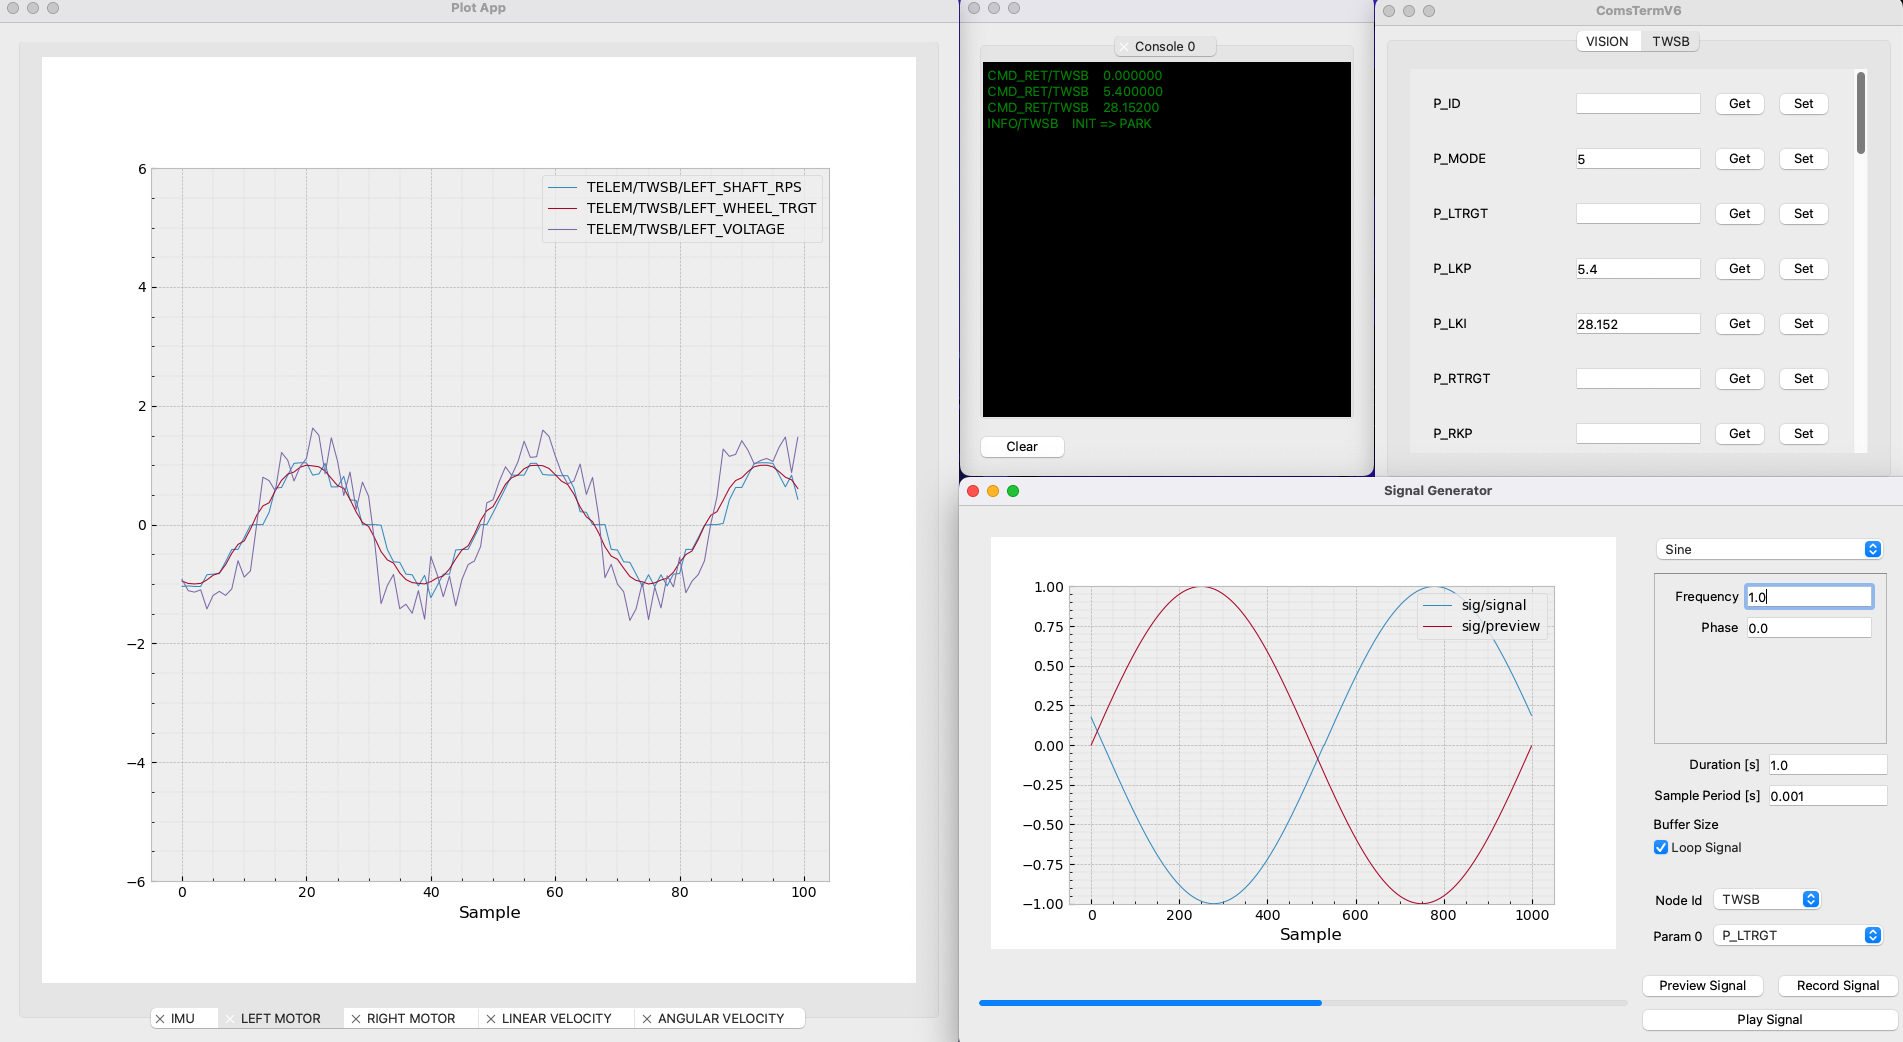
\includegraphics[height=0.45\textwidth]{SysIDMotorSetUp.png}
            \caption{System Identification Testbench Setup}
            \label{fig:SysIDSetUp}
        \end{figure}
        The test suit contains a timeseries signal generators, with preview and playback functionality.
        The Systems logs and messages are displayed in a terminal window, and the user is able to fully configure 
        each nodes runtime parameters remotely over a network connection, utilizing the RPC ASCII protocol.
        A line plotter, is configured by JSON to display any number of signals.
        This architecture allows for repeatability in obtaining robot data, something 
        is is a challenge in mobile robotics[]. 
        
        This software system is also utilized for huristic tuning of the control
        and vision systems. The program is able to visualize control signal streams in soft real time, 
        and provides a useful insight into the effects of the control system on the plant.

        \begin{figure}[H]
            \centering
            \begin{subfigure}[b]{0.45\textwidth}
            \includegraphics[width=\textwidth]{Graphs/openstep.pdf}
            \caption{Open Loop Step Response}
            \label{fig:openstep}
            \end{subfigure}
            \hfill
            \begin{subfigure}[b]{0.45\textwidth}
            \includegraphics[width=\textwidth]{Graphs/1HzSine.pdf}
            \caption{Open Loop Sine Response}
            \label{fig:opensine}
            \end{subfigure}
            \caption{Open Loop no Load Speed Voltage Experiments}
            \label{fig:openloop}
        \end{figure}


        From these experiments it is clear that the motor is has significant deadzones, 
        and the input output relationship is non linear at low speeds. When the motor is operating at its rated currnet, 
        seen by the experiments in \ref{fig:speedvolt}, its its linearity is improved. The maximum no load speed is  
        \begin{figure}[H]
            \centering
            \includegraphics[width=0.5\textwidth]{Graphs/SpeedVoltageCurve.pdf}
            \caption{Speed Voltage Relationship}
            \label{fig:speedvolt}
        \end{figure}

        This non-linearity is a result of the motors backlash, which is a common issue in low cost gearboxes.
        \cite{grasser2002joe} utilizes a low pass filter to mitigate some of the more sever effects of 
        this deadline; mechanical vibration increased thermal stress and noise. 
        In the case of the TWSB system, when it is stationary, 
        the actuators will not be static and are required to be operating mostly is a sinusoidal version, 
        similar to \ref{fig:opensine} in order to regulate the pitch angle of the body.
        Considering this a closed loop controller is developed in section 4.1 to regulate the motors speed,
         and maintain the device is it operating region. 
    \pagebreak{}



    \section{State Estimation}
    Information about a system may be obtained from 2 types of sources; 
    mathematical models models as in eq(1) which can describe the time evolution of the chosen system variables, 
    and sensors that convert energy arising from a physical property into information[]. Both of which are approximation of the true state. 
    The process of combining multiple sources of information is termed sensor fusion.

    \subsection{Sensors Overview}
        For the TWSB system in eq(6) its state variables $\theta$ and $\dot x_b$ can be measured by the onboard IMU and the wheel encoders.
        The motors incorporates a low cost 12 pulses per revolution (ppr) quadrature encoder. The hardware decoder peripheral on the MCU
        is used to increment the pulse count and the rotational speed is updated at each step of a fixed rate loop[].
        
        The IMU is a 6 axis MEMS sensor[] which measures the local linear acceleration 
        and angular velocity.
        The 3D acceleration $\vec{a}$ is used to obtain an 
        estimate of the pitch angle as    $\hat{\theta} = \mathrm{atan2}\left(-a_x ,a_z \right)$

        The variance of this $\hat{\theta}$ is small when the system is at rest, but grows larger when subject to vibration from the motors
        as shown by the experiment in \ref{fig:accelNoise} where the TWSB is placed horizontally at rest and motor control commands are issued. 
        \begin{figure}[H]
            \centering
            \begin{subfigure}[b]{0.5\textwidth}

                \includegraphics[width=\textwidth]{Graphs/accelNoiseReadings.pdf}
                \caption{Accelerometer is sensitive to motor vibrations}
                \label{fig:accelRaw}
                
            \end{subfigure}
            \hfill
            \begin{subfigure}[b]{0.45\textwidth}
                \includegraphics[width=\textwidth]{Graphs/noisyPitchEst.pdf}
                \caption{Wide Variance on pitch estimate at rest}
                \label{fig:pitchNoise}
            \label{fig:accelNoise}
            \end{subfigure}
            \caption{Accelerometer Noise}   
        \end{figure}

        From \ref{fig:pitchNoise} it can be seen that the IMU is not mounted perfectly orthogonal to the body frame. 
        \begin{table}[H]
            \centering
            \begin{tabular}{c c c} 
                \toprule
                $a_{x_0}$ & $a_{y_0}$ & $a_{z_0}$ \\
                \midrule
                0.036453 & -0.0021066 & 0.133658 \\
                \bottomrule

            \end{tabular}
            \caption{Accelerometer Mounting Offset (m/s$^{2}$)}
            \label{tab:accelOffset}
        \end{table}
        This systematic error is removed by utilizing calibrated values in table obtained as per \ref{tab:accelOffset}.
        
        
        \pagebreak{}
        \subsection{Kalman Filter}
        The Kalman Filter (KF) and its variants  are widely used in robotics to fuse 
        complementary sources of information \cite{Thrun2005ProbabilisticRobotics} \cite{perez2023quadcopter} \cite{Moore2014AGE}.
        The ordinary KF is applicable to linear systems, as a type of Bayesian filter, 
        the discreet representation of the KF represents current belief $bel(x_k)$ around the true state,
        as a Gaussian whose distribution is parameterized by its mean $\mu_k$ and covariance matrix $P_k$.

        A new measurement is observed at each timestamp through the linear function $z_k = C_k x_k + R_k$. 
        The measurement model $C_k$ is used to map the true state into the measurement space.
        Here the process and measurement noise are Gaussian with zero mean and covariance $Q_k$ and $R_k$ respectively. 
        The Kalman Gain computed as \ref{eq:KalmanGain} provides the optimal weighting between t
        he beliefs from the prediction \ref{eq:KalmanPredict} and the measurement update \ref{eq:KalmanUpdate}.
        

        \begin{subequations}
            \begin{equation}
                \bar{bel}(x_k) = \begin{cases}
                        \bar{\mu}_k = F_k \mu_{k-1} + G_k u_k \\
                        \bar{P}_k = F_k P_{k-1} F_k^T + Q_k
                        \end{cases}
                \label{eq:KalmanPredict}
            \end{equation}
            \begin{equation}
                K_k = \bar{P_k} C_k^T \left(C_k \bar{P_k} C_k^T + R_k \right)^{-1}
                \label{eq:KalmanGain}
            \end{equation}
            \begin{equation}
            bel(x_k) = \begin{cases}
                \mu_k = \bar{\mu}_k + K_k \left(z_k - C_k \bar{\mu}_k \right) \\
                P_k = \left(I - K_k C_k \right) \bar{P}_k
            \end{cases}
            \label{eq:KalmanUpdate}
            \end{equation}
            \label{eq:KalmanAlgorithm}
        \end{subequations}
     
        Even though the state transition model of the TWSB robot is non-linear
        \cite{ooi2003balancing} 
        developed self balancing platforms capable of restricting oscillations about the 
        operating point to $±1$ degree. This one order of magnitude than the worst case pitch limit of $±10$ degrees.
        Beyond this, the small angle approximation is no longer valid, and the system is not locally linear. 

        The state transition model used by the KF, can be choses to model the TWSB system \ref{eq:2DOF} as a step towards 
        full state feedback, or solely the dynamics of the IMU.  Both approaches have had success in the literature[][][]. 
        An alternative approach is to use a simplification of the noise modeling used by classical baysian saticitcs and 
        assume that the noise covariance are time invariant, the complementary filter \cite{ComplimentaryKalman} 
        is a popular choice for this due to its low mathematical complexity. 
     
        An early work on  attitude control of the TWSB system by \cite{SelfContainedMobileTWSB} directly integrates the gyroscope and its bias 
        and despite the bias drift, is able to be stabilized whilst moving. 
        The MPU6050 6-Axis IMU can estimate the pitch through the gyroscope measurement $\vec\omega_{gyro}$ and the accelerometer measurement $\vec a_{x}$.

        \begin{equation}
            \begin{aligned}
                \begin{bmatrix}
                    \theta_{g{k}} \\
                    \beta_{k} 
                \end{bmatrix}
                &= 
                \begin{bmatrix}
                    1 & -\Delta t \\
                    0 & 1
                \end{bmatrix}
                \begin{bmatrix}
                    \theta_{g{k-1}} \\
                    \beta_{k-1}
                \end{bmatrix}
                +
                \begin{bmatrix}
                    \Delta t \\
                    0
                \end{bmatrix}
                + \begin{bmatrix}
                    -\rho_{k-1}\cdot\Delta t \\
                    \rho_b
                \end{bmatrix}
            \end{aligned}
            \label{eq:gyroBias1}
        \end{equation}
        
        \begin{equation}
            \begin{aligned}
                z_k &= \begin{bmatrix}
                    1 & 0
                \end{bmatrix}
                \begin{bmatrix}
                    \theta_k \\
                    \nu_{g{k}}
                \end{bmatrix}
                + \begin{bmatrix}
                    \rho_{a{k}}
                \end{bmatrix}
            \end{aligned}
            \label{eq:gyroBias2}
        \end{equation}
        

        \begin{figure}[H]
            \centering
            \includegraphics[width=0.8\textwidth]{Graphs/SensorFusion.pdf}
            \caption{Sensor Fusion of accelerometer and gyroscope}
            \label{fig:SensorFusion}
        \end{figure}

        The MPU6050 parameters are obtained from the dataset[] as 
        \begin{table}[H]
            \centering
            \begin{tabular}{|c|c|c|}
                \hline
                Parameter & Value & Units \\
                \hline
                $a_{sensitivity}$ & 16384 & LSB/g \\
                $g_{sensitivity}$ & 131 & LSB/deg/s \\
                \hline
            \end{tabular}
            \caption{MPU6050 Parameters}
        \end{table}
        The kalman gain matrix is obtained operating the motors to simulate typical high frequency conditions 
        and tuning the process and measurement noise matrices.
        \begin{table}[H]
            \centering
            \begin{tabular}{|c|c|c|}
                \hline
                Parameter & Value & Units \\
                \hline
                $Q$ & 0.01 & $rad^2$ \\
                $R$ & 0.01 & $rad^2$ \\
                \hline
            \end{tabular}
            \caption{Kalman Filter Noise Parameters}
        \end{table}

       
        \ref{fig:SensorFusion} shows that the Kalman Filter's produces a smooth estimate of the pitch angle
        under conditions of the experiment in \ref{fig:accelNoise}. It is observed that when there is a 
        large change in the motors set-point  the angular momentum built up from the wheels is sufficient to 
        disturb the system from rest seen at $k \approx [170, 380, 580]$.
        \pagebreak{}
    \section{Control System}
        Autonomy in mobile robotics is commonly a hierarchical problem, composed of high level path planning, 
        or task allocation,and low level control of the actuators, successful implementations must design 
        solutions to both of these probelms in a complementary manner. 
               
        \cite{patle2019review} reviews planning strategies implemented in the mobile robotics literature. 
        The choice of strategy is found to be dependant on the available hardware and modeling complexity. 
        \cite{yamamoto2008nxtway} develops a high fidelity model and simulation study of a WIP platform 
        using low cost sensors and actuators, yet is able to achieve a high level of performance.
        Conversely a simpler PID regulator is used by [] as the robot is fitted with brushless motors
        which can be readily torque controlled. 
        In cases where the goal is to achieve high levels of autonomy, [][] use sliding mode 
        control in order to utilize  aggressively tuned various controllers for different requirements and 
        automatically and smoothly switch between these.

        Parameter uncertainty is a common issue in controlling mobile robotics, and approximations of these often lead to 
        discrepancies between the mathematical optimal solutions found in simulation \cite{eide2011lqg} 
        and in real world performance. This often leads to designers experimentally tuning algorithms. These kinds of 
        feedback algorithms perform purely reactive corrections; an error measurement 
        is required at each time step to compute the control law, $u$. By nature of this, the signals utilized in these 
        regulators often have direct physical relations to the plant, providing intuition to the designer for initial values through 
        elementary unit analysis. For example the input-outut data of the sleected actuators obtained in \ref{fig:openloop}, 
        one can natruly see that a large inegral action is needed to overcome the steady state error at low speeds, since the 
        open loop plants resonse is of the same shape as the referencc, the propotinal and derivative constants in the velocity PID
        algorithm formualted in descreet time as 

            
        Will have a much smaller effect of the close loop response. 
        Methods such as Ziegler-Nichols formulate approaches to black-box tuning of a plant through observing the systems 
        performance under sustained sustained instability. Whilst providing a systematic tuning strategy performance validation 
        in the model-free cases such as the PID algorithm must be evaluated at runtime, 
        thus in cases of unstable or safety critical systems common in process control[][].
        
        To this end, the field of adaptive control proposes dealing with these uncertainties by designing controllers which may learn 
        by online trial-and-error data,  statistical teqchcinies like regression based transfer function estimated form of
        input-output data. physics informed models taken under statistical distributions of belief. \cite{benosman2018model}. 
    
        However in the case of unstable systems, can be destructive,


        
            
        \cite{williams2016aggressive} in a similar vein embeds
        a neural network as an online function approximate to learn predictions of the systems dynamics. 
        This prediction is then used as part of a trajectory planner in race-line optimization. 

        Some modern microcontroler have sufficient computational power requirements needed for Model Predictive Control (MPC) and 
        effective imprecations of such optimizers have been used in small mobile robots \cite{nguyen2024tinympc}. 

        An attractive aspect of predictive approaches to control is that they lend themselves naturally to 
        planning long horizons, or tasks. These methods utilizes numeral simulation techniques to evolve the system 
        over time stimate the distibutions of state probabilites from a monte-calrlo sampling of control actions. The optimal
        contol sequence is then chosen from these samples through a cost fucntion. 
        

        
        The autonomous behavior of the TWSB 
        robot explored in this paper is that of path following in an unknown environment, where no prior 
        map is available. As such the control system has 3 goals, namely disturbance rejection of the
        pitch angle; this is required such that the system is robust to the environment, 
        regulating of linear velocity set-points, so the TWSB location in its body frame is controlled, 
        and tracking a trajectory obtained by a high level planner discussed in section 6. 

        A simple PID controller operating on the pitch error is tested in simscape multibody; 
        a physics based siulation where the control law 
        is an applided force to a prismatic joint. This force is coupled through the revolute 
        joint to the pitch angle as descried by \ref{eq:2DOF}.
        This manages to stabilize the pitch angle however as shown by fig, x position drifts.

        The TWSB achieves balance by controlling the oscillations of the pitch angle about the 
        vertical axis. The linearized system of equations in \ref{eq:2DOF} is applicable 
        only when the pitch angle is small, this is taken to be $\theta < ±10$ degrees. 
 
        In the sequence the low level controls are developed to meet these requirements:
        \begin{enumerate}
            \item The pitch angle must be regulated to $±1$ degree.
            \item The global $x$ position should be controlled by a linear velocity reference.
        \end{enumerate}
        allowing for teleoperation where a operator is tasked with the navigation of the robot. 






        \subsection{Cascade PID}
        Since the linear velocity is coupled to the
        pitch angle, the target pitch angle must be controlled to maintain a constant x velocity. 
        This is achieved by regulating the pitch angle about equilibrium. In cascade control, the term main process varibale 
        is usuauly the o

        This approach in theory, should also be a able to mitigate the effects of mounting offset of the IMU, by desining the outerloop
        to correct in the long term position drift induced by the faster dynamics of the inner balacing loop.

        A cascaded pid controller is used to control the pitch angle and the linear velocity. 
        Control of the position $(x_g,y_g)$ is left to a higher level planner.  
        If the inner loop dynamics are much faster than the outer loop, 
        then the inner loop can be approximated as a disturbance[].

        In order to determine the maximum operating frequency of the outer loop, 
        the inner motor speed loop is closed at 200Hz and the system is observed.
        
        Through the Ziegler-Nichols method[], the PID gains for each DC Motors speed control loop 
        are obtained as shown in table(2). This process however may cause damage to the motors 
        during the sustained oscillations at the critical gain. 
       
        The frequency response of the transfer function is shown in fig(4) 
        and its closed loop bandwidth is determined to be ... rads

        This is then used to obtain the PID gains in table(4) in MATLAB using pole-placement techniques
        \begin{table}[H]
            \centering
            \begin{tabular}{|c|c|c|}
                \hline
                Parameter & Zeigler-Nichols & SysId \\
                \hline 
                $K_p$ & 0.1 & 0.1 \\
                $K_i$ & 0.01 & 0.01 \\
                $K_d$ & 0.01 & 0.01 \\
                \hline
            \end{tabular}
            \caption{PID Gains}
        \end{table}

        A P controller is used to regulate the steering control signal, which modeled
        as a disturbance from the 2D dynamics model.

        The error of the pitch angle is regulated by a PID controller operating at 100Hz. 
        
        This results in a stable system in 1DOF space, controlling the body velocity requires the outermost loop to be closed at 20Hz.
        The final cascaded closed loop pid controller is shown in fig(5) with the gains in table(5)

        \begin{figure}[H]
            \includegraphics[width=\textwidth]{Diagrams/cascade.pdf}
            \caption{Cascaded PID Controller}
        \end{figure}

        \begin{table}[H]
            \centering
            \begin{tabular}{|r|r|r|r|c|c|c|c}
                \hline
                & \multicolumn{5}{c|}{Process Variable}  \\
                \hline
                Parameter & $v_b$ & $\theta$  & $\omega_L$ & $\omega_R$ & $\dot{\psi_b}$ \\
                \hline      
                $K_p$ & 2.2 & 0.19 & 2.4 & 2.9 & 0.8 \\
                $K_i$ & 0.8 & 5.6 & 24.8 & 24.8 & 2\\
                $K_d$ & 0 & 0.003 & 0 & 0  &  0\\
                \hline
            \end{tabular}
            \caption{PID Gains}
        \end{table}
        \pagebreak{}
        \subsection{LQR}
        A Linear Quadratic Regulator (LQR) is used to control the system in 2DOF space.
        This minimizes 
        
       
        Selecting the Q and R matrixes as eq(7) and eq(8) respectively, 
        the K feedback matrix in eq(9) is obtained by solving the Algebraic Riccati
        equation of the discretized system eq(10) in MATLAB.
        sample frequency determine based on rise time of simulated closed loop model. 
        by Nyquist the system must then be sampled at least 200Hz. 

        \pagebreak{}
        \section{Vision System}

        Map building is a popular approach for navigation as it allows for a large 
        context of the environment to be considered and guarantees can be made such as obstacle avoidance and optimal path selection \cite{Macenski_2020}. 

        \subsection{Camera Sensor}

        \subsubsection{Calibration}

        \subsection{Robust Line Detection Algorithms}

        \subsection{Navigation requirements}

        \subsection{Indoor Drivability Segmentation}

        \subsection{Racing Algorithms}

        \subsection{Predictive Trajectory Generation}
    
    \pagebreak{}


  %%%%%%%%%%%%%%%%%% SECTION 4 %%%%%%%%%%%%%%%%%%
  \section{Results and discussion} % edit section heading as appropriate
    \subsection{Balance Performance}

    \subsection{Operational Robustness}
    \subsection{Line Trajectory Tracking}
    \begin{figure}[H]
        \centering
        \begin{subfigure}[c]{0.35\textwidth}
            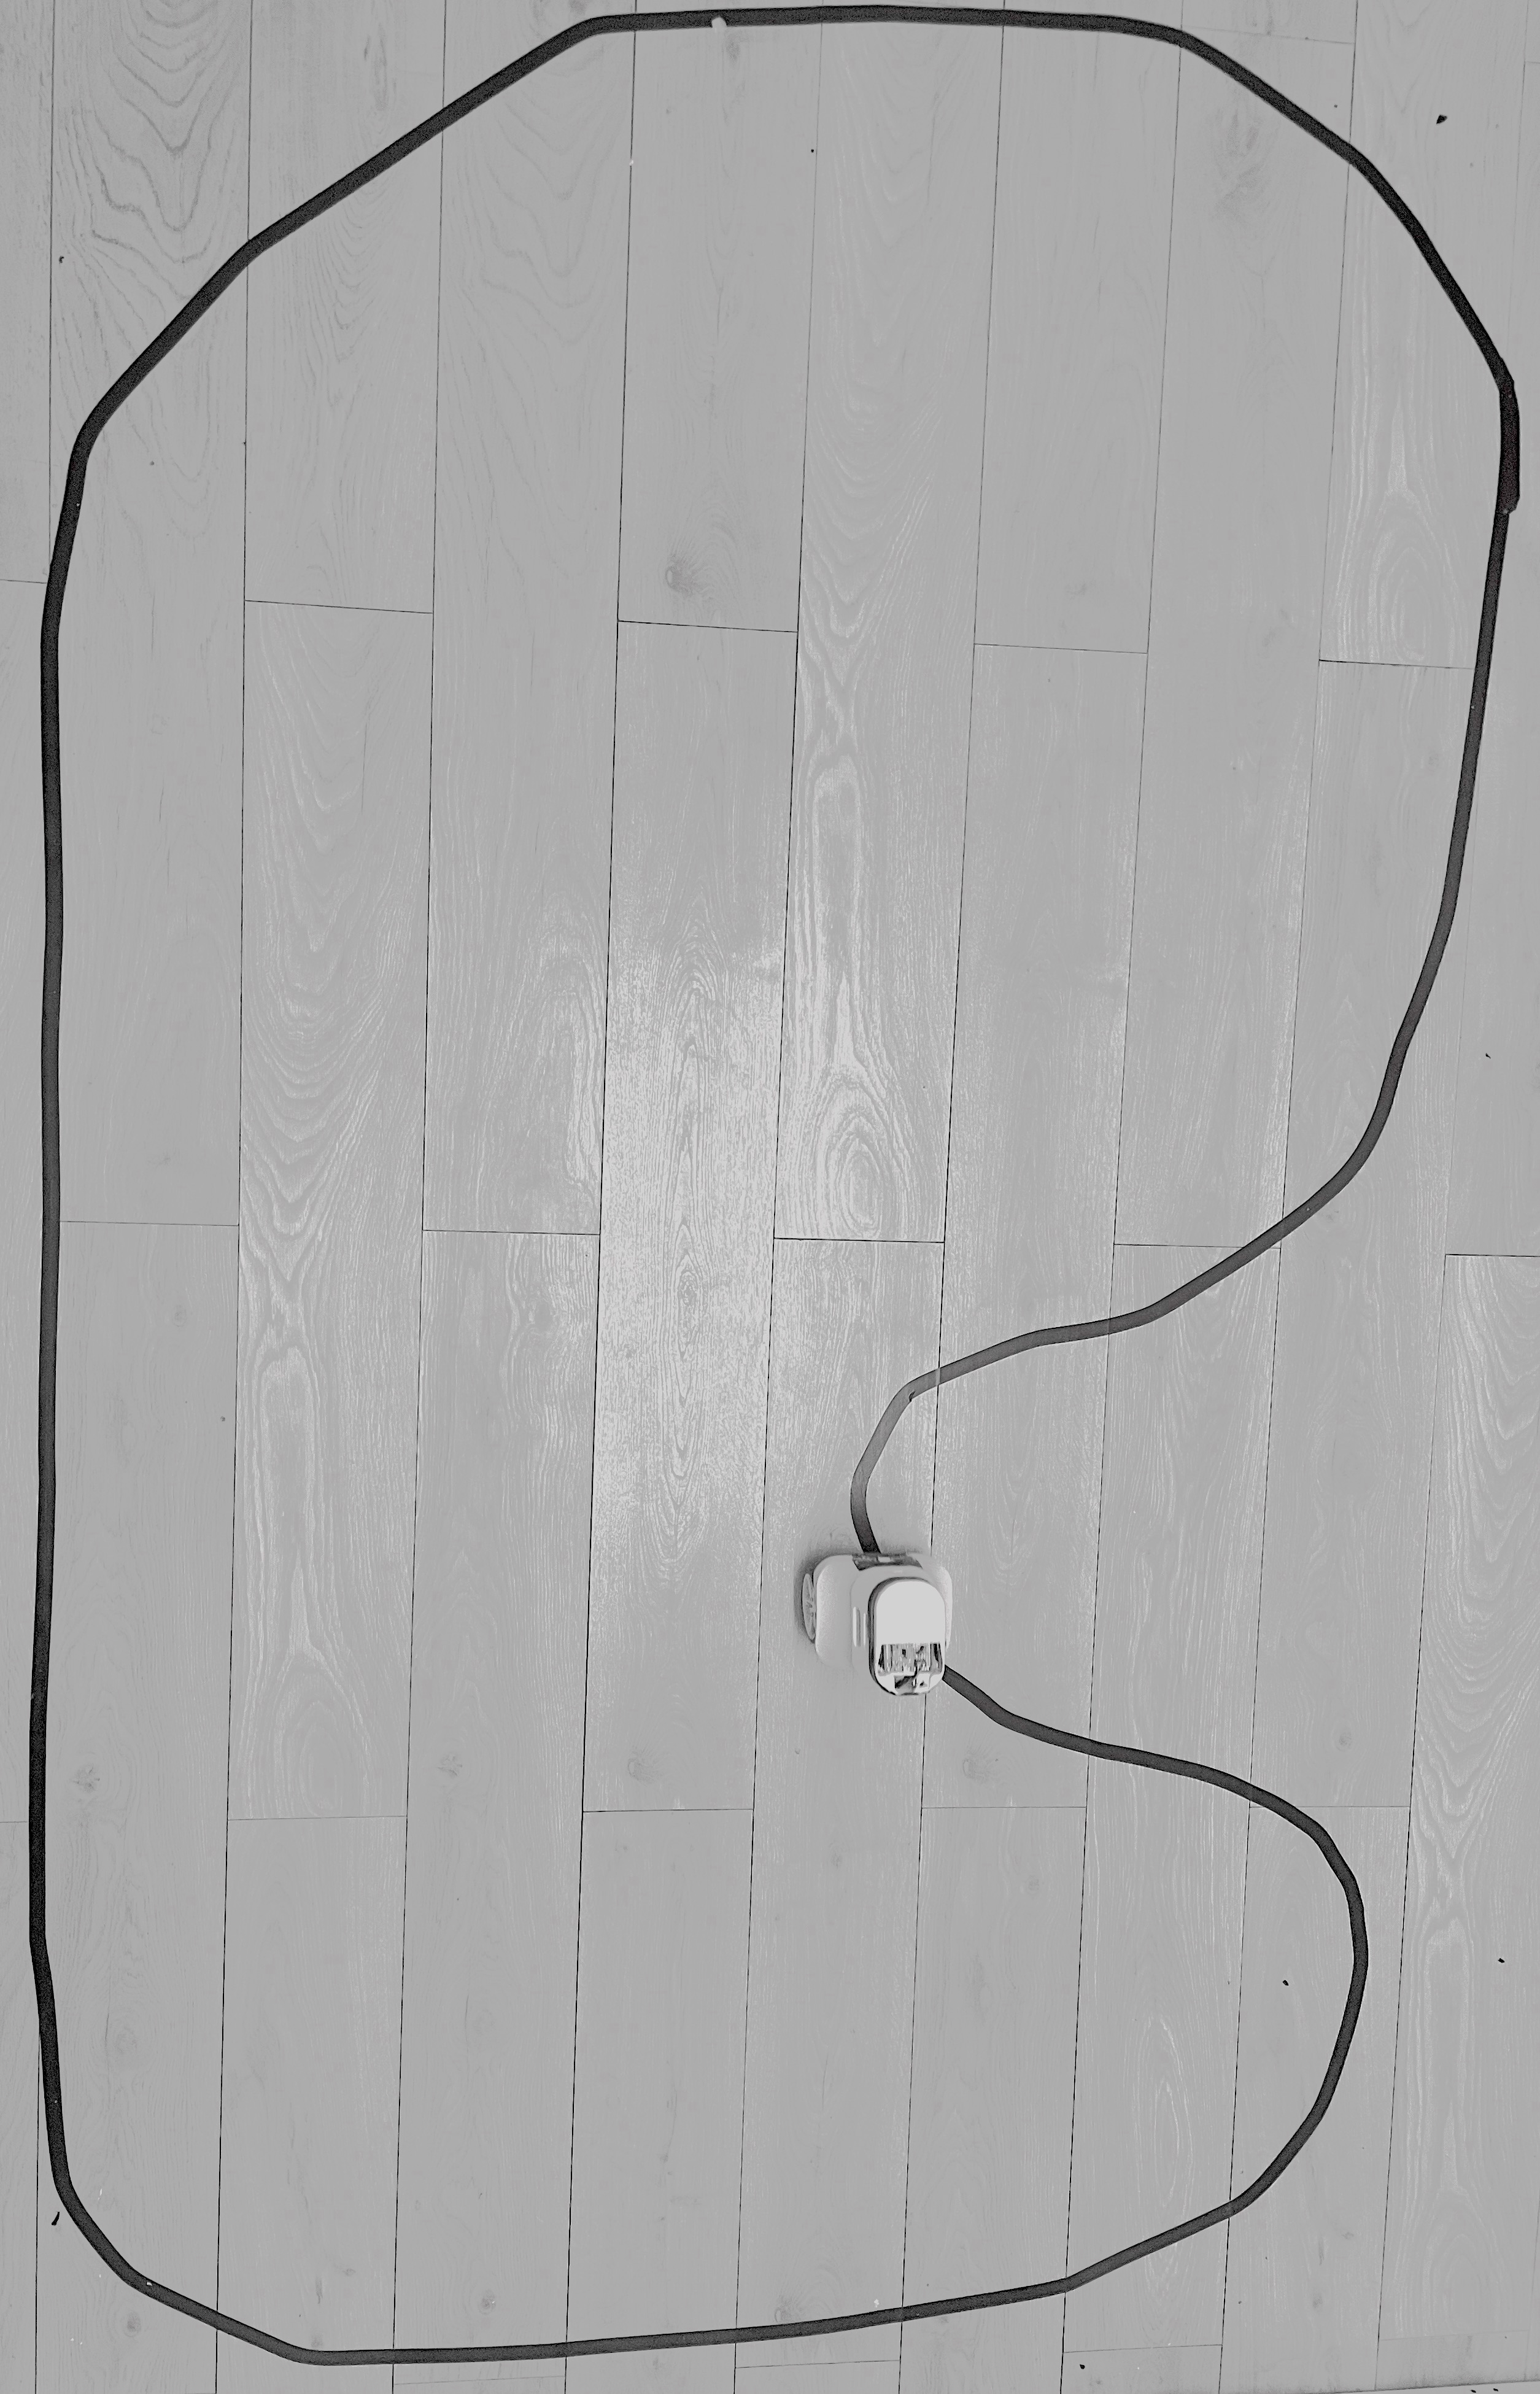
\includegraphics[height=1.3\textwidth]{TrajTrak.jpeg}
            \caption{Race Track}
        \end{subfigure}
        \hfill
        \begin{subfigure}[c]{0.6\textwidth}
            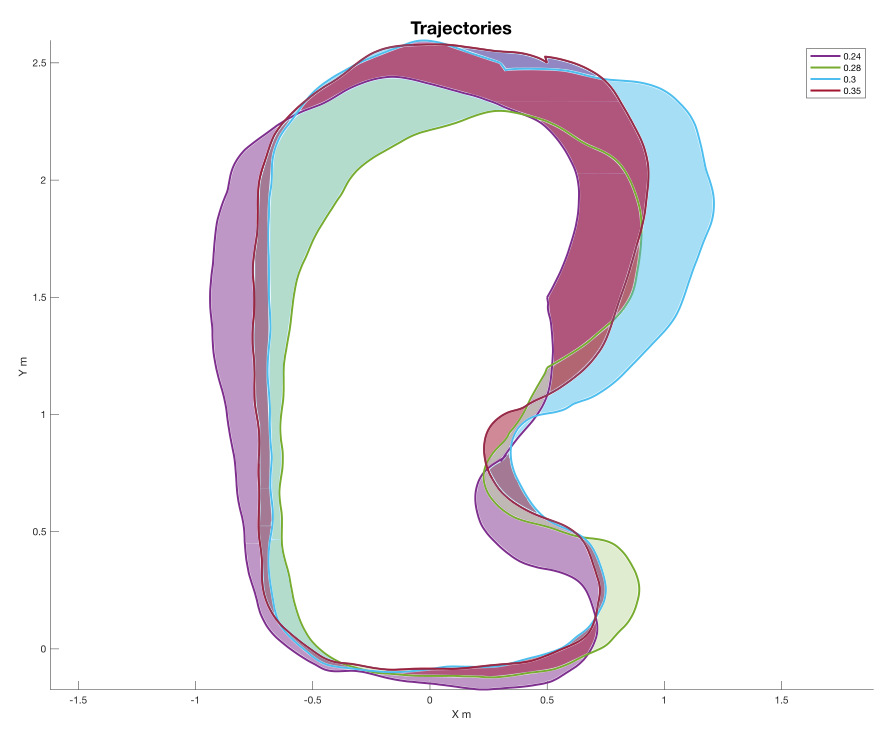
\includegraphics[width=1.2\textwidth]{Graphs/DeadReckoningTrackMap.png}

            \caption{Map built offline using dead reckoning}
        \end{subfigure}
        \caption{Trajectory Tracking and Map Visualization}
        \label{fig:TrajTrack}
    \end{figure}
    \subsection{More detail}
    \subsection{Summary}
  %%%%%%%%%%%%%%%%%% SECTION 5 %%%%%%%%%%%%%%%%%%
  \section{Conclusions and future work} % edit section heading as appropriate
    \subsection{Conclusions}
      \subsection{Future work}
  %%%%%%%%%%%%%%%%%% REFERENCES %%%%%%%%%%%%%%%%%%
    \printbibliography
  %%%%%%%%%%%%%%%%%% APPENDICES %%%%%%%%%%%%%%%%%%
  \begin{uomappendix} 
      \section{Code}
      \section{Risk assessment}
      Risk assessment is a required appendix. Put here.
      %\section{Other appendices as necessary}
  \end{uomappendix}
  
  %%%%%%%%%%%%%%%%%% END MATTER %%%%%%%%%%%%%%%%%%
  \end{document}